\chapter{overvied of CADAL data}
What I was able to do:
    My findings:
        * There exists enough data in the CADAL set to compare many of the same characters, attributed to the same author, across a variety of texts.
        *  Many of the characters encoded in CADAL Calligraphy many characters are single specimens and therefore defy individual comparisons.  The Chinese language contains a vast variety of characters, many of which are used infrequently.
        *  The CADAL character set provides positional data for a only a very small portion: probably less than 10\% of retrieved calligraphy pages.  (Need Statistics here)
        *  Of the pages with CADAL character positional information, a significant portion of the characters present are not reflected in the character database.
    
    \begin{figure}{}
    \parbox{12cm}{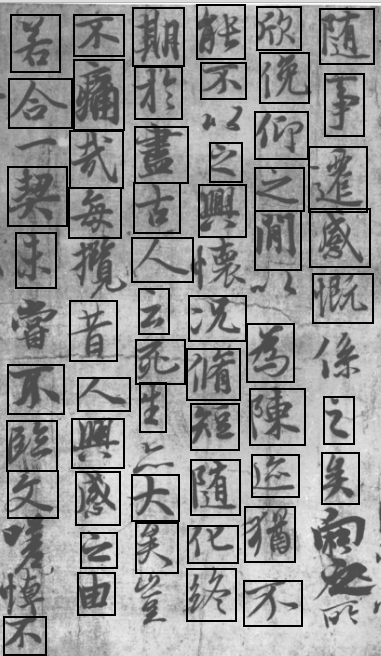
\includegraphics[width=12cm]{cadal-most-characters-boxed.png}}
    \caption{This page has bounding box data for most characters}
    \label{cadal most characters boxed}
    \end{figure}
    
    \begin{figure}{}
    \parbox{12cm}{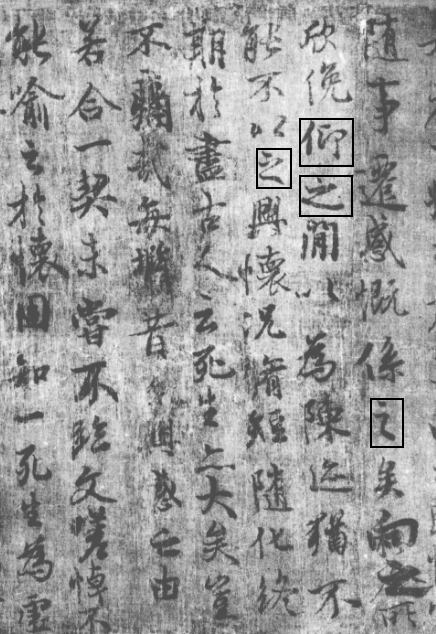
\includegraphics[width=12cm]{cadal-few-characters-boxed.png}}
    \caption{This page have bounding box data for very few characters}
    \label{cadal less characters boxed}
    \end{figure}
    
    \begin{figure}{}
    \parbox{12cm}{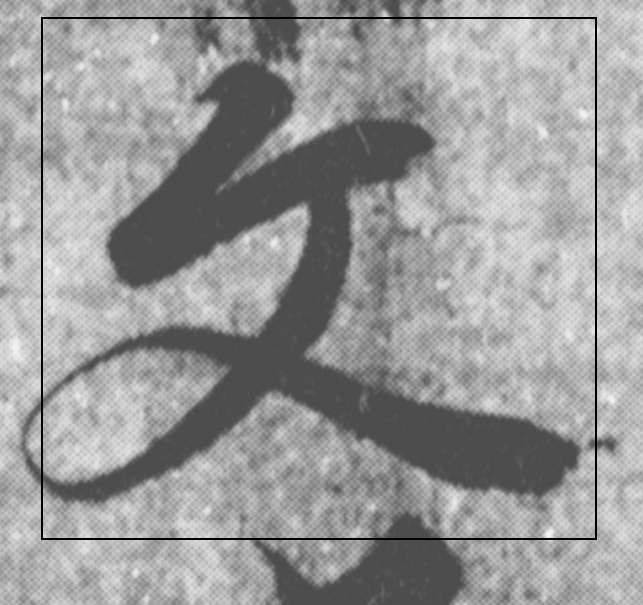
\includegraphics[width=12cm]{cadal-box-missing-part-of-character.png}}
    \caption{Box not covering whole character, and box overlaps a different character when it doesn't have to}
    \label{cadal single character examples}
    \end{figure}
    
    \begin{figure}{}
    \parbox{12cm}{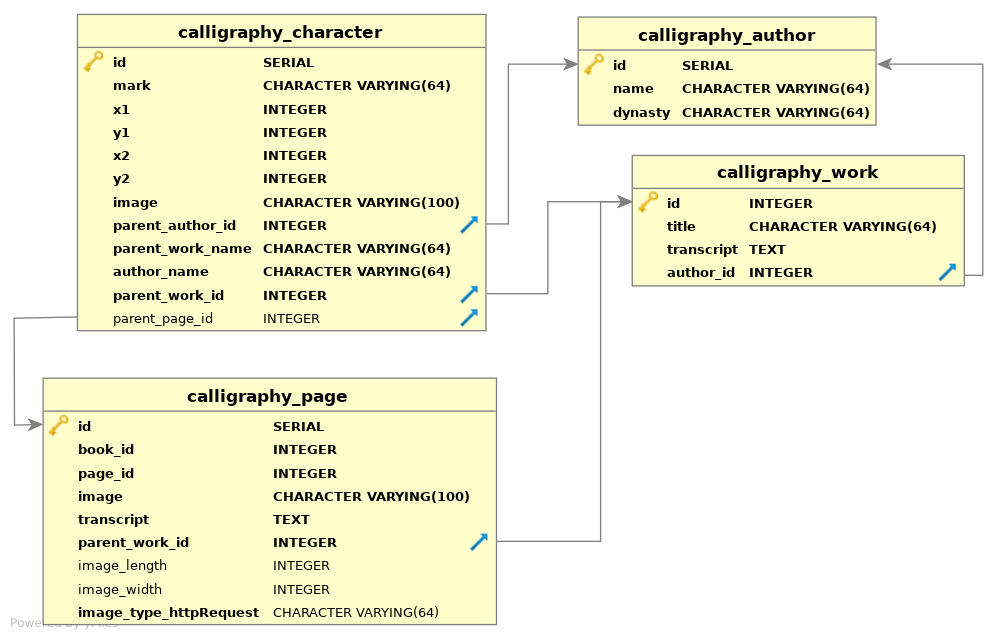
\includegraphics[width=12cm]{calliset-erd.png}}
    \caption{character database in calliset website}
    \label{character database in calliset website}
    \end{figure}
    
